% Options for packages loaded elsewhere
\PassOptionsToPackage{unicode}{hyperref}
\PassOptionsToPackage{hyphens}{url}
%
\documentclass[
  english,
  doc,floatsintext]{apa6}
\usepackage{amsmath,amssymb}
\usepackage{lmodern}
\usepackage{ifxetex,ifluatex}
\ifnum 0\ifxetex 1\fi\ifluatex 1\fi=0 % if pdftex
  \usepackage[T1]{fontenc}
  \usepackage[utf8]{inputenc}
  \usepackage{textcomp} % provide euro and other symbols
\else % if luatex or xetex
  \usepackage{unicode-math}
  \defaultfontfeatures{Scale=MatchLowercase}
  \defaultfontfeatures[\rmfamily]{Ligatures=TeX,Scale=1}
\fi
% Use upquote if available, for straight quotes in verbatim environments
\IfFileExists{upquote.sty}{\usepackage{upquote}}{}
\IfFileExists{microtype.sty}{% use microtype if available
  \usepackage[]{microtype}
  \UseMicrotypeSet[protrusion]{basicmath} % disable protrusion for tt fonts
}{}
\makeatletter
\@ifundefined{KOMAClassName}{% if non-KOMA class
  \IfFileExists{parskip.sty}{%
    \usepackage{parskip}
  }{% else
    \setlength{\parindent}{0pt}
    \setlength{\parskip}{6pt plus 2pt minus 1pt}}
}{% if KOMA class
  \KOMAoptions{parskip=half}}
\makeatother
\usepackage{xcolor}
\IfFileExists{xurl.sty}{\usepackage{xurl}}{} % add URL line breaks if available
\IfFileExists{bookmark.sty}{\usepackage{bookmark}}{\usepackage{hyperref}}
\hypersetup{
  pdftitle={Early Biomarkers of Parkinson's Disease Based on Natural Connected Speech},
  pdfauthor={Anja Probst1},
  pdflang={en-EN},
  pdfkeywords={keywords},
  hidelinks,
  pdfcreator={LaTeX via pandoc}}
\urlstyle{same} % disable monospaced font for URLs
\usepackage{color}
\usepackage{fancyvrb}
\newcommand{\VerbBar}{|}
\newcommand{\VERB}{\Verb[commandchars=\\\{\}]}
\DefineVerbatimEnvironment{Highlighting}{Verbatim}{commandchars=\\\{\}}
% Add ',fontsize=\small' for more characters per line
\usepackage{framed}
\definecolor{shadecolor}{RGB}{248,248,248}
\newenvironment{Shaded}{\begin{snugshade}}{\end{snugshade}}
\newcommand{\AlertTok}[1]{\textcolor[rgb]{0.94,0.16,0.16}{#1}}
\newcommand{\AnnotationTok}[1]{\textcolor[rgb]{0.56,0.35,0.01}{\textbf{\textit{#1}}}}
\newcommand{\AttributeTok}[1]{\textcolor[rgb]{0.77,0.63,0.00}{#1}}
\newcommand{\BaseNTok}[1]{\textcolor[rgb]{0.00,0.00,0.81}{#1}}
\newcommand{\BuiltInTok}[1]{#1}
\newcommand{\CharTok}[1]{\textcolor[rgb]{0.31,0.60,0.02}{#1}}
\newcommand{\CommentTok}[1]{\textcolor[rgb]{0.56,0.35,0.01}{\textit{#1}}}
\newcommand{\CommentVarTok}[1]{\textcolor[rgb]{0.56,0.35,0.01}{\textbf{\textit{#1}}}}
\newcommand{\ConstantTok}[1]{\textcolor[rgb]{0.00,0.00,0.00}{#1}}
\newcommand{\ControlFlowTok}[1]{\textcolor[rgb]{0.13,0.29,0.53}{\textbf{#1}}}
\newcommand{\DataTypeTok}[1]{\textcolor[rgb]{0.13,0.29,0.53}{#1}}
\newcommand{\DecValTok}[1]{\textcolor[rgb]{0.00,0.00,0.81}{#1}}
\newcommand{\DocumentationTok}[1]{\textcolor[rgb]{0.56,0.35,0.01}{\textbf{\textit{#1}}}}
\newcommand{\ErrorTok}[1]{\textcolor[rgb]{0.64,0.00,0.00}{\textbf{#1}}}
\newcommand{\ExtensionTok}[1]{#1}
\newcommand{\FloatTok}[1]{\textcolor[rgb]{0.00,0.00,0.81}{#1}}
\newcommand{\FunctionTok}[1]{\textcolor[rgb]{0.00,0.00,0.00}{#1}}
\newcommand{\ImportTok}[1]{#1}
\newcommand{\InformationTok}[1]{\textcolor[rgb]{0.56,0.35,0.01}{\textbf{\textit{#1}}}}
\newcommand{\KeywordTok}[1]{\textcolor[rgb]{0.13,0.29,0.53}{\textbf{#1}}}
\newcommand{\NormalTok}[1]{#1}
\newcommand{\OperatorTok}[1]{\textcolor[rgb]{0.81,0.36,0.00}{\textbf{#1}}}
\newcommand{\OtherTok}[1]{\textcolor[rgb]{0.56,0.35,0.01}{#1}}
\newcommand{\PreprocessorTok}[1]{\textcolor[rgb]{0.56,0.35,0.01}{\textit{#1}}}
\newcommand{\RegionMarkerTok}[1]{#1}
\newcommand{\SpecialCharTok}[1]{\textcolor[rgb]{0.00,0.00,0.00}{#1}}
\newcommand{\SpecialStringTok}[1]{\textcolor[rgb]{0.31,0.60,0.02}{#1}}
\newcommand{\StringTok}[1]{\textcolor[rgb]{0.31,0.60,0.02}{#1}}
\newcommand{\VariableTok}[1]{\textcolor[rgb]{0.00,0.00,0.00}{#1}}
\newcommand{\VerbatimStringTok}[1]{\textcolor[rgb]{0.31,0.60,0.02}{#1}}
\newcommand{\WarningTok}[1]{\textcolor[rgb]{0.56,0.35,0.01}{\textbf{\textit{#1}}}}
\usepackage{graphicx}
\makeatletter
\def\maxwidth{\ifdim\Gin@nat@width>\linewidth\linewidth\else\Gin@nat@width\fi}
\def\maxheight{\ifdim\Gin@nat@height>\textheight\textheight\else\Gin@nat@height\fi}
\makeatother
% Scale images if necessary, so that they will not overflow the page
% margins by default, and it is still possible to overwrite the defaults
% using explicit options in \includegraphics[width, height, ...]{}
\setkeys{Gin}{width=\maxwidth,height=\maxheight,keepaspectratio}
% Set default figure placement to htbp
\makeatletter
\def\fps@figure{htbp}
\makeatother
\setlength{\emergencystretch}{3em} % prevent overfull lines
\providecommand{\tightlist}{%
  \setlength{\itemsep}{0pt}\setlength{\parskip}{0pt}}
\setcounter{secnumdepth}{-\maxdimen} % remove section numbering
% Make \paragraph and \subparagraph free-standing
\ifx\paragraph\undefined\else
  \let\oldparagraph\paragraph
  \renewcommand{\paragraph}[1]{\oldparagraph{#1}\mbox{}}
\fi
\ifx\subparagraph\undefined\else
  \let\oldsubparagraph\subparagraph
  \renewcommand{\subparagraph}[1]{\oldsubparagraph{#1}\mbox{}}
\fi
% Manuscript styling
\usepackage{upgreek}
\captionsetup{font=singlespacing,justification=justified}

% Table formatting
\usepackage{longtable}
\usepackage{lscape}
% \usepackage[counterclockwise]{rotating}   % Landscape page setup for large tables
\usepackage{multirow}		% Table styling
\usepackage{tabularx}		% Control Column width
\usepackage[flushleft]{threeparttable}	% Allows for three part tables with a specified notes section
\usepackage{threeparttablex}            % Lets threeparttable work with longtable

% Create new environments so endfloat can handle them
% \newenvironment{ltable}
%   {\begin{landscape}\begin{center}\begin{threeparttable}}
%   {\end{threeparttable}\end{center}\end{landscape}}
\newenvironment{lltable}{\begin{landscape}\begin{center}\begin{ThreePartTable}}{\end{ThreePartTable}\end{center}\end{landscape}}

% Enables adjusting longtable caption width to table width
% Solution found at http://golatex.de/longtable-mit-caption-so-breit-wie-die-tabelle-t15767.html
\makeatletter
\newcommand\LastLTentrywidth{1em}
\newlength\longtablewidth
\setlength{\longtablewidth}{1in}
\newcommand{\getlongtablewidth}{\begingroup \ifcsname LT@\roman{LT@tables}\endcsname \global\longtablewidth=0pt \renewcommand{\LT@entry}[2]{\global\advance\longtablewidth by ##2\relax\gdef\LastLTentrywidth{##2}}\@nameuse{LT@\roman{LT@tables}} \fi \endgroup}

% \setlength{\parindent}{0.5in}
% \setlength{\parskip}{0pt plus 0pt minus 0pt}

% Overwrite redefinition of paragraph and subparagraph by the default LaTeX template
% See https://github.com/crsh/papaja/issues/292
\makeatletter
\renewcommand{\paragraph}{\@startsection{paragraph}{4}{\parindent}%
  {0\baselineskip \@plus 0.2ex \@minus 0.2ex}%
  {-1em}%
  {\normalfont\normalsize\bfseries\itshape\typesectitle}}

\renewcommand{\subparagraph}[1]{\@startsection{subparagraph}{5}{1em}%
  {0\baselineskip \@plus 0.2ex \@minus 0.2ex}%
  {-\z@\relax}%
  {\normalfont\normalsize\itshape\hspace{\parindent}{#1}\textit{\addperi}}{\relax}}
\makeatother

% \usepackage{etoolbox}
\makeatletter
\patchcmd{\HyOrg@maketitle}
  {\section{\normalfont\normalsize\abstractname}}
  {\section*{\normalfont\normalsize\abstractname}}
  {}{\typeout{Failed to patch abstract.}}
\patchcmd{\HyOrg@maketitle}
  {\section{\protect\normalfont{\@title}}}
  {\section*{\protect\normalfont{\@title}}}
  {}{\typeout{Failed to patch title.}}
\makeatother
\keywords{keywords\newline\indent Word count: X}
\usepackage{csquotes}
\ifxetex
  % Load polyglossia as late as possible: uses bidi with RTL langages (e.g. Hebrew, Arabic)
  \usepackage{polyglossia}
  \setmainlanguage[]{english}
\else
  \usepackage[main=english]{babel}
% get rid of language-specific shorthands (see #6817):
\let\LanguageShortHands\languageshorthands
\def\languageshorthands#1{}
\fi
\ifluatex
  \usepackage{selnolig}  % disable illegal ligatures
\fi
\newlength{\cslhangindent}
\setlength{\cslhangindent}{1.5em}
\newlength{\csllabelwidth}
\setlength{\csllabelwidth}{3em}
\newenvironment{CSLReferences}[2] % #1 hanging-ident, #2 entry spacing
 {% don't indent paragraphs
  \setlength{\parindent}{0pt}
  % turn on hanging indent if param 1 is 1
  \ifodd #1 \everypar{\setlength{\hangindent}{\cslhangindent}}\ignorespaces\fi
  % set entry spacing
  \ifnum #2 > 0
  \setlength{\parskip}{#2\baselineskip}
  \fi
 }%
 {}
\usepackage{calc}
\newcommand{\CSLBlock}[1]{#1\hfill\break}
\newcommand{\CSLLeftMargin}[1]{\parbox[t]{\csllabelwidth}{#1}}
\newcommand{\CSLRightInline}[1]{\parbox[t]{\linewidth - \csllabelwidth}{#1}\break}
\newcommand{\CSLIndent}[1]{\hspace{\cslhangindent}#1}

\title{Early Biomarkers of Parkinson's Disease Based on Natural Connected Speech}
\author{Anja Probst\textsuperscript{1}}
\date{}


\shorttitle{Biomarkers of Parkinson's Disease}

\authornote{

The authors made the following contributions. Anja Probst: Conceptualization, Writing - Original Draft Preparation, Writing - Review \& Editing.

Correspondence concerning this article should be addressed to Anja Probst, 24 rue du Général-Dufour, 1211 Genève 4. E-mail: \href{mailto:anja.probst@etu.unige.ch}{\nolinkurl{anja.probst@etu.unige.ch}}

}

\affiliation{\vspace{0.5cm}\textsuperscript{1} University of Geneva}

\abstract{
Parkinson's Disease is a degenerative disorder of the nervous system that
globally affects more than 6 million people (\url{doi:10.1016/S0140-6736(16)31678-6}).
While the most well-recognized symptoms of the disease are motor-related, such
as shaking and instability, a further group of symptoms, which is only partially motor-related
and occurs in a majority of patients, are speech-altering symptoms (\url{https://pubmed.ncbi.nlm.nih.gov/30223711/}).
While the disease is well-recognizable at a later stage, it is exceptionally hard to diagnose
and differentiate in its early stages and appropriate treatment is often delayed.
In 2017, Hlavnička et al.~have published a study suggesting that automated analysis of connected
speech can reveal early biomarkers in subjects with REM sleep behaviour disorder, who are at
high risk of developing Parkinson's disease. In this project I analyse the data set published by
the authors that contains experimental evaluation of healthy controls (HC, \(n=50\)), subjects with REM
sleep behaviour disorder (RBD, \(n=50\)), and subjects with Parkinson's Disease (PD, \(n=30\)). While the constraints
of this project limit the scope of analysis, I will show that interesting insights into the data can be
gained nontheless.
}



\begin{document}
\maketitle

\clearpage

\hypertarget{introduction}{%
\section{Introduction}\label{introduction}}

\hypertarget{context-of-the-project}{%
\subsection{Context of the Project}\label{context-of-the-project}}

Patients with the neurodegenerative disease Parkinson's have numerous symptoms ranging from cognitive
impairments to motor symptoms. Those symptoms may appear relatively late in the disease when the
neurodegeneration has already widely spread in different areas of the brain (mainly Basal Ganglia).
Main symptoms of PD are motor dysfunctions including abnormalities in the production and sound of
speech of such patients (up to 90\%). These abnormalities in speech and voice are called hypokinetic
dysarthria which is characterized by a decreased quality of the speech, where the voice, sound formation
as well as the articulation is impaired. As I mentioned before, often motor impairments are detected
relatively late in the disease. To improve diagnostics and to detect the disease in a much earlier stage,
the detection of biomarkers related to neurodegeneration could lead to a better prognosis and therapy of PD.

Therefore, the investigation of prodromal speech changes could be an appropriate and suitable approach.
To investigate this approach, an automated speech monitoring system was developed, that uses a
segmentation method for the precise estimation of voiced and unvoiced segments of speech, respirations,
and pauses. Further proposed was a set of acoustic speech features based on the segmentation algorithm
applicable to connected speech, allowing the description of complex vocal disturbances due to neurodegeneration
including respiratory deficits, dysphonia, imprecise articulation, and dysrhythmia.

In this data analysis project, the main focus was to explore, if there are any speech patterns that
support the usage of an automated speech monitoring system to detect prodromal parkinsonian
neurodegeneration based on natural connected speech.

130 subjects were tested. 30 subjects with early, untreated Parkinson's disease (PD) where the disease
is already manifested. 50 subjects with REM sleep behaviour disorder (RBD), which is a disease where
its relatively likely to develop PD in a later phase. As a control group, 50 healthy subjects (HD) were included.

\hypertarget{manual-variable-selection}{%
\subsection{Manual Variable Selection}\label{manual-variable-selection}}

Due to the constraints of this project, I reduced the data set from originally 62 variables to the best fitting 7.
As I am looking specificially into the aspect of speech, and to evaluate if speech is a good predictor for PD,
I chose speech related variables that were assessed empirically and were reported to have the most significant differences
between healthy controls and subjects with early stages of Parkinson's Disease.
Note that patient group will be extracted from the variable Participant\_code.
The resulting data set is summarized in Table~\ref{tab:summarize-data-frame}

\begin{Shaded}
\begin{Highlighting}[]
\NormalTok{cols.to.keep }\OtherTok{\textless{}{-}} \FunctionTok{c}\NormalTok{(}
    \StringTok{"Participant\_code"}\NormalTok{, }\StringTok{"Age"}\NormalTok{, }\StringTok{"Gender"}\NormalTok{, }\StringTok{"Rate\_of\_speech\_timing"}\NormalTok{,}
    \StringTok{"Rate\_of\_speech\_timing.1"}\NormalTok{, }\StringTok{"Duration\_of\_pause\_intervals"}\NormalTok{,}
    \StringTok{"Duration\_of\_pause\_intervals.1"}
\NormalTok{)}

\CommentTok{\# Above columns will be renamed to}
\NormalTok{rename.cols.to }\OtherTok{\textless{}{-}} \FunctionTok{c}\NormalTok{(}
    \StringTok{"Participant\_code"}\NormalTok{, }\StringTok{"Age"}\NormalTok{, }\StringTok{"Gender"}\NormalTok{, }\StringTok{"Speech.Timing.Rate.Reading"}\NormalTok{,}
    \StringTok{"Speech.Timing.Rate.Monologue"}\NormalTok{, }\StringTok{"Pause.Interval.Duration.Reading"}\NormalTok{,}
    \StringTok{"Pause.Interval.Duration.Monologue"}
\NormalTok{)}

\NormalTok{csv.path }\OtherTok{\textless{}{-}} \StringTok{"BiomarkersPD.csv"}
\NormalTok{df }\OtherTok{\textless{}{-}} \FunctionTok{read.csv}\NormalTok{(csv.path, }\AttributeTok{sep =} \StringTok{","}\NormalTok{, }\AttributeTok{header =} \ConstantTok{TRUE}\NormalTok{)}

\CommentTok{\# Only keep required columns and rename them}
\NormalTok{df }\OtherTok{\textless{}{-}}\NormalTok{ df[cols.to.keep]}
\FunctionTok{colnames}\NormalTok{(df) }\OtherTok{\textless{}{-}}\NormalTok{ rename.cols.to}

\CommentTok{\# Replace "{-}" with NA}
\NormalTok{df[df }\SpecialCharTok{==} \StringTok{"{-}"}\NormalTok{] }\OtherTok{\textless{}{-}} \ConstantTok{NA}

\CommentTok{\# Get groups from participant codes by replacing numerical values}
\NormalTok{df}\SpecialCharTok{$}\NormalTok{Group }\OtherTok{\textless{}{-}} \FunctionTok{gsub}\NormalTok{(}\StringTok{"[[:digit:]]+"}\NormalTok{, }\StringTok{""}\NormalTok{, df}\SpecialCharTok{$}\NormalTok{Participant\_code)}

\CommentTok{\# Participant codes no longer required, remove}
\NormalTok{df }\OtherTok{\textless{}{-}} \FunctionTok{subset}\NormalTok{(df, }\AttributeTok{select =} \SpecialCharTok{{-}}\FunctionTok{c}\NormalTok{(Participant\_code))}

\CommentTok{\# Convert columns to factors}
\NormalTok{col.names }\OtherTok{\textless{}{-}} \FunctionTok{c}\NormalTok{(}\StringTok{"Group"}\NormalTok{, }\StringTok{"Gender"}\NormalTok{)}
\NormalTok{df[col.names] }\OtherTok{\textless{}{-}} \FunctionTok{lapply}\NormalTok{(df[col.names], as.factor)}
\end{Highlighting}
\end{Shaded}

\hypertarget{data-description}{%
\subsection{Data Description}\label{data-description}}

For each sample in this data set (\(n=130\)), we have the following information:

\begin{itemize}
\tightlist
\item
  Demographic information:

  \begin{itemize}
  \tightlist
  \item
    Age (years)
  \item
    Gender (M for male, F for female)
  \end{itemize}
\item
  Speech examination - Speaking task of reading passage: speakers read a standardized, phonetically-balanced text of 80 words twice

  \begin{itemize}
  \tightlist
  \item
    Duration\_Of\_Pause\_Intervals\_Reading: Duration of pause intervals (DPI) describes the quality of speech timing, as pauses can be heavily influenced by the ability to properly initiate speech, it is measured in miliseconds (ms)
  \item
    Rate\_Of\_Speech\_Timing\_Reading: Rate of speech time (RST) includes voiced, unvoiced and pause intervals, it is measured in intervals per minute (-/min)
  \end{itemize}
\item
  Speech examination - Speaking task of monologue: participants were instructed to provide monologue about their interests, job, family or current activities for approximately 90 seconds

  \begin{itemize}
  \tightlist
  \item
    Duration\_Of\_Pause\_Intervals\_Monologue: Duration of pause intervals (DPI) describes the quality of speech timing, as pauses can be heavily influenced by the ability to properly initiate speech, it is measured in milliseconds (ms)
  \item
    Rate\_Of\_Speech\_Timing\_Monologue: Rate of speech time (RST) includes voiced, unvoiced and pause intervals, it is measured in intervals per minute (-/min)
  \end{itemize}
\item
  Group: based on Participant Code

  \begin{itemize}
  \tightlist
  \item
    PD: subjects with Parkinson's disease
  \item
    RBD: subjects with REM sleep behaviour disorder
  \item
    HC: healthy controls
  \end{itemize}
\end{itemize}

\begin{table}[!htbp] \centering \renewcommand*{\arraystretch}{1.1}\caption{Summary of the Data Set used in this Analysis}\label{tab:summarize-data-frame}\resizebox{\textwidth}{!}{
\begin{tabular}{lrrrrrrr}
\hline
\hline
Variable & N & Mean & Std. Dev. & Min & Pctl. 25 & Pctl. 75 & Max \\ 
\hline
Age & 130 & 64.331 & 10.134 & 34 & 58.25 & 72 & 83 \\ 
Gender & 130 &  &  &  &  &  &  \\ 
... F & 27 & 20.8\% &  &  &  &  &  \\ 
... M & 103 & 79.2\% &  &  &  &  &  \\ 
Speech.Timing.Rate.Reading & 130 & 327.277 & 47.385 & 140 & 297.25 & 358.75 & 457 \\ 
Speech.Timing.Rate.Monologue & 130 & 288.338 & 52.892 & 112 & 258 & 328.75 & 412 \\ 
Pause.Interval.Duration.Reading & 130 & 166.646 & 46.488 & 96 & 138.25 & 185 & 388 \\ 
Pause.Interval.Duration.Monologue & 130 & 229.069 & 79.697 & 117 & 177 & 263.25 & 611 \\ 
Group & 130 &  &  &  &  &  &  \\ 
... HC & 50 & 38.5\% &  &  &  &  &  \\ 
... PD & 30 & 23.1\% &  &  &  &  &  \\ 
... RBD & 50 & 38.5\% &  &  &  &  & \\ 
\hline
\hline
\end{tabular}
}
\end{table}

\begin{verbatim}
'data.frame':   130 obs. of  7 variables:
 $ Age                              : int  58 68 68 75 61 58 79 59 73 66 ...
 $ Gender                           : Factor w/ 2 levels "F","M": 1 1 2 2 2 2 2 1 2 2 ...
 $ Speech.Timing.Rate.Reading       : int  354 340 211 140 269 317 269 338 374 281 ...
 $ Speech.Timing.Rate.Monologue     : int  333 285 247 112 230 181 289 370 288 258 ...
 $ Pause.Interval.Duration.Reading  : int  146 173 377 360 211 186 214 145 117 213 ...
 $ Pause.Interval.Duration.Monologue: int  158 295 280 397 206 611 251 118 194 246 ...
 $ Group                            : Factor w/ 3 levels "HC","PD","RBD": 2 2 2 2 2 2 2 2 2 2 ...
\end{verbatim}

\clearpage

\hypertarget{data-pre-processing}{%
\section{Data Pre-Processing}\label{data-pre-processing}}

As an initial step, I created boxplots to check the distribution of the numerical data per group
in detail (Figure \ref{fig:boxplots-and-correlations}).
At first glance, parts of the data show skewed distributions, as the mean (shown as a orange point)
differs substantially in many cases. This might prompt data transformations such as the \(log\)-transform.
Additionally, within each variable, the distributions between the groups were assessed for significant differences.
Here, the data showed significant differences between healthy controls (HC) and Parkinson's (PD) and REM sleep
behaviour disorder subjects (RBD), but no significant differences between PD and RBD. Based on this, I decided
to split the data anlysis part into two sections: (1) Creating a logistic regression model using \texttt{glm} to
discriminate between the two groups HC and PD and (2) creating a multinomial regression model which discriminates
between all three groups (HC, PD, and RBD).

\begin{figure}

{\centering 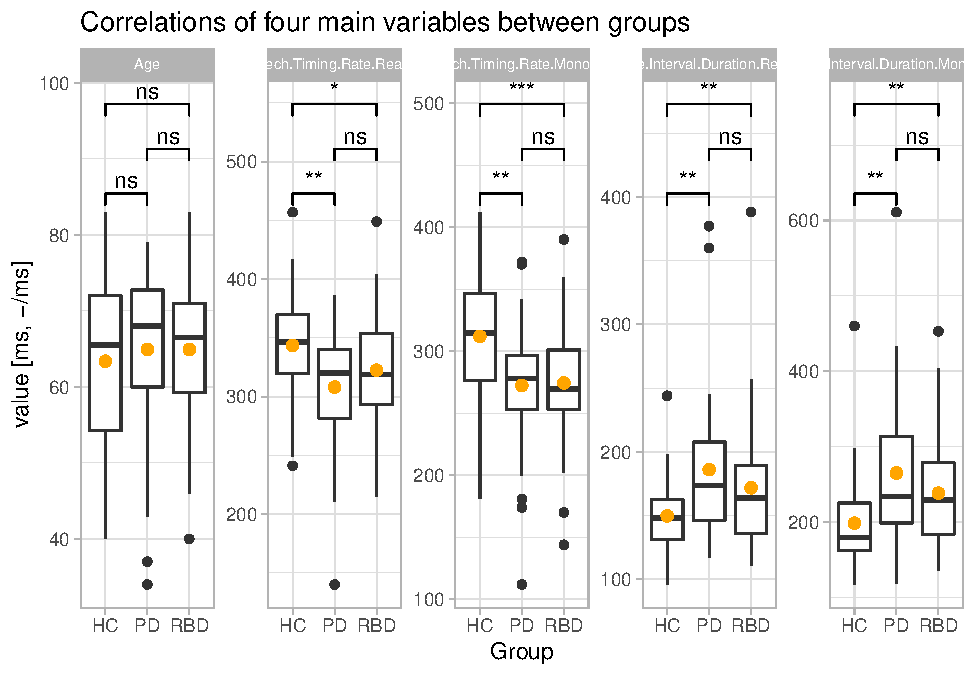
\includegraphics{dap_report_anja_probst_files/figure-latex/boxplots-and-correlations-1} 

}

\caption{Distributions of data within variables and between groups. Some of the data shows skewed distributions (mean is represented by orange point), especially within the variable Age. While there is significant difference (t-Test) between healthy controls (HC) and subjects with Parkinson's disease (PD) as well as REM sleep behavior disorder (RBD), there are no significant differences between PD and RBD}\label{fig:boxplots-and-correlations}
\end{figure}

Based on the empirical variables chosen, I excpected them to correlate. Indeed, Figure \ref{fig:correlate-ggpairs-plot} shows
a relatively strong correlation between these variables. Based on visual inspection of the boxplots (Figure \ref{fig:boxplots-and-correlations}), I chose to remove outliers
in the following way:

\begin{figure}

{\centering 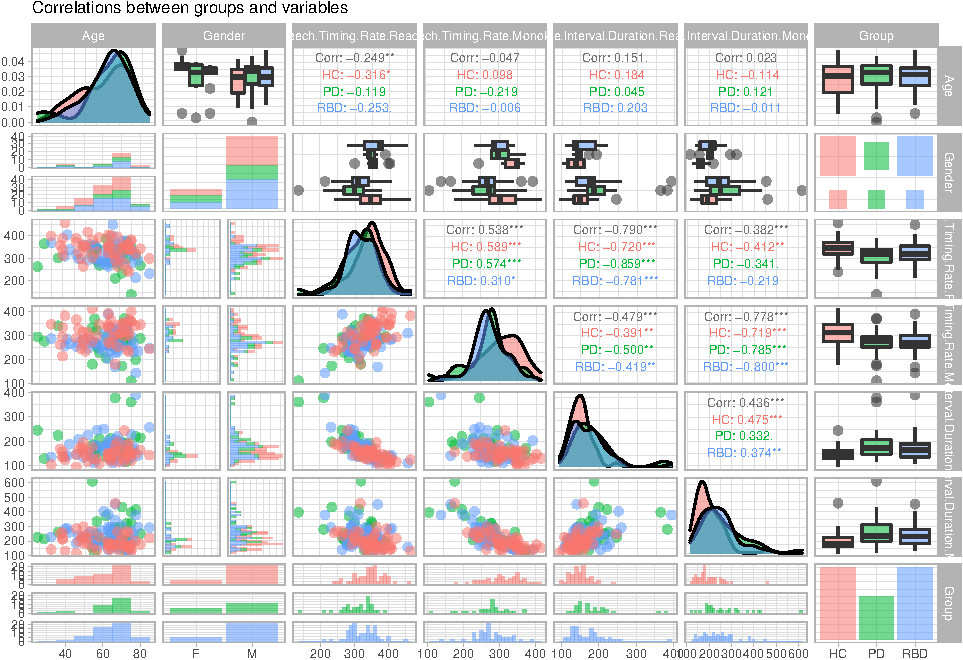
\includegraphics{dap_report_anja_probst_files/figure-latex/correlate-ggpairs-plot-1} 

}

\caption{Plot based on ggpairs, colored by the response variable Group. The empirically collected speech data shows strong correlations (both positive and negative). In addition the density plots show the skewed distributions that were already seen in the boxplots.}\label{fig:correlate-ggpairs-plot}
\end{figure}

\begin{Shaded}
\begin{Highlighting}[]
\NormalTok{df }\OtherTok{\textless{}{-}}\NormalTok{ df[df}\SpecialCharTok{$}\NormalTok{Pause.Interval.Duration.Monologue }\SpecialCharTok{\textless{}} \DecValTok{600}\NormalTok{, ]}
\NormalTok{df }\OtherTok{\textless{}{-}}\NormalTok{ df[(df}\SpecialCharTok{$}\NormalTok{Group }\SpecialCharTok{!=} \StringTok{"HC"} \SpecialCharTok{|}\NormalTok{ df}\SpecialCharTok{$}\NormalTok{Pause.Interval.Duration.Monologue }\SpecialCharTok{\textless{}} \DecValTok{450}\NormalTok{), ]}
\end{Highlighting}
\end{Shaded}

Given a lack of correlation between age and any of the speech-related variables, I chose to not remove
outliers based on the variable age.

\clearpage

\hypertarget{data-analysis}{%
\section{Data Analysis}\label{data-analysis}}

\hypertarget{logistic-regression}{%
\subsection{Logistic Regression}\label{logistic-regression}}

As stated previously, I have seen that there are no significant differences between the groups PD and RBD.
Based on this observation, I will limit my initial investigation to creating a logistic regression model predicting
between the groups HC and PD. Indeed, the paper from which the data was extracted explicitly
discusses the hard problem of differentiating PD from RBD, which might very well be impossible with
generalised linear models. I will revisit this problem in the section Multinomial Regression.

As a first step, a subset is created that does not contain any observations from the group RBD.

\begin{Shaded}
\begin{Highlighting}[]
\NormalTok{df.binom }\OtherTok{\textless{}{-}} \FunctionTok{data.frame}\NormalTok{(df[df}\SpecialCharTok{$}\NormalTok{Group }\SpecialCharTok{!=} \StringTok{"RBD"}\NormalTok{, ])}
\end{Highlighting}
\end{Shaded}

Based on this subset, I first create simple logistic regression models with one response variable
for each of the selected variables (Figure \ref{fig:simple-logistic-regression}). For simplicity
they were created using the \texttt{ggplot2} function \texttt{stat\_smooth}. As can be seen by visual inspection
of the data points (red), none of the predictors is sufficient to predict the response variable
(Group) on its own, given the respective overlap between the two groups.

\begin{figure}

{\centering 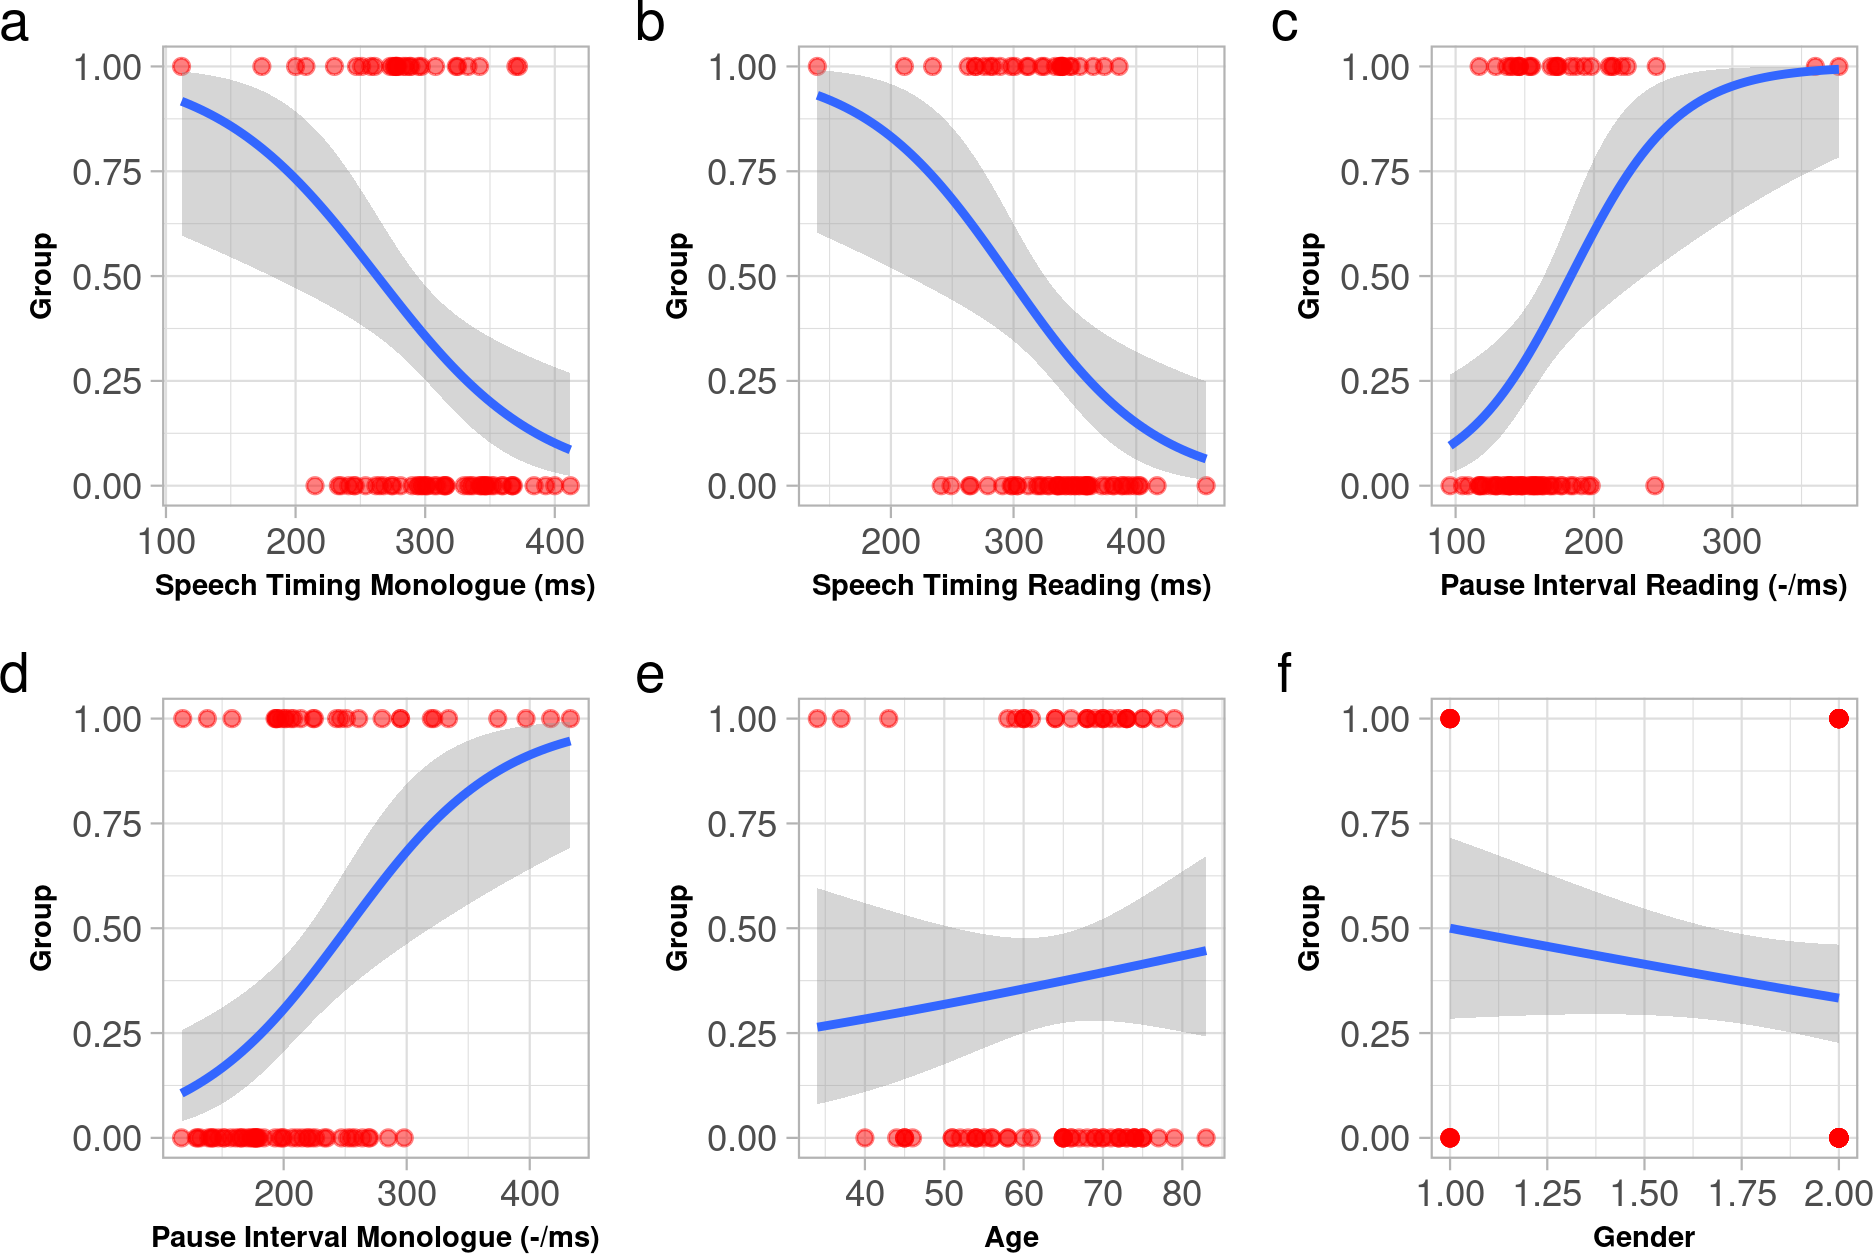
\includegraphics{dap_report_anja_probst_files/figure-latex/simple-logistic-regression-1} 

}

\caption{Simple logistic regression models with one predictor each. For variables a to d, we can see a clear sigmoid curve, while variables e, and of course f, which is a factor, do not show such a curve.}\label{fig:simple-logistic-regression}
\end{figure}

Given that a single predictor is clearly not sufficient, a series of multiple logistic regression models
have to be built and evaluated. As I would have to test 64 models (all possible combinations plus
intercept only) to be certain to have found the best one, I instead chose to use the automated model
selection function \texttt{dredge} from the R package \texttt{MuMIn}. Starting from the global binomial model
\texttt{Group\ \textasciitilde{}\ .} as an input, \texttt{dredge} enumerates all possible models and evaluates them based on their AIC.

\begin{Shaded}
\begin{Highlighting}[]
\NormalTok{m.full }\OtherTok{\textless{}{-}} \FunctionTok{glm}\NormalTok{(}
    \AttributeTok{data =}\NormalTok{ df.binom, Group }\SpecialCharTok{\textasciitilde{}}\NormalTok{ .,}
    \AttributeTok{family =}\NormalTok{ binomial,}
    \AttributeTok{na.action =} \StringTok{"na.fail"}
\NormalTok{)}

\NormalTok{d }\OtherTok{\textless{}{-}} \FunctionTok{dredge}\NormalTok{(m.full, }\AttributeTok{rank =} \StringTok{"AIC"}\NormalTok{)}

\NormalTok{m.best.no.interactions }\OtherTok{\textless{}{-}} \FunctionTok{get.models}\NormalTok{(d, }\DecValTok{1}\NormalTok{)[[}\DecValTok{1}\NormalTok{]]}
\FunctionTok{summary}\NormalTok{(m.best.no.interactions)}
\end{Highlighting}
\end{Shaded}

\begin{table}[tbp]

\begin{center}
\begin{threeparttable}

\caption{\label{tab:table-best-model-dredge}A full regression table of the best model (selected using dredge) without interactions.}

\begin{tabular}{lllll}
\toprule
Predictor & \multicolumn{1}{c}{$b$} & \multicolumn{1}{c}{95\% CI} & \multicolumn{1}{c}{$z$} & \multicolumn{1}{c}{$p$}\\
\midrule
Intercept & -5.53 & {}[-8.93, -2.73] & -3.50 & < .001\\
GenderM & -1.79 & {}[-3.22, -0.49] & -2.61 & .009\\
Pause Interval Duration Monologue & 0.01 & {}[0.00, 0.03] & 2.33 & .020\\
Pause Interval Duration Reading & 0.02 & {}[0.00, 0.04] & 1.98 & .048\\
\bottomrule
\end{tabular}

\end{threeparttable}
\end{center}

\end{table}

Importantly, the above automated model selection did not consider interactions between the predictors.
Given the strong collinearity of the model (based the relatively strong correlation between the speech-related
variables) it would be interesting to see whether solely the interaction between two variables would provide
a better model. Indeed, the model below shows that solely focusing on the interactions provides a better result.

\begin{table}[tbp]

\begin{center}
\begin{threeparttable}

\caption{\label{tab:interaction-model}A full regression table of a manually created model with based on an interaction between the variables Pause Interval Duration Reading and Pause Interval Duration Monologue.}

\begin{tabular}{lllll}
\toprule
Predictor & \multicolumn{1}{c}{$b$} & \multicolumn{1}{c}{95\% CI} & \multicolumn{1}{c}{$z$} & \multicolumn{1}{c}{$p$}\\
\midrule
Intercept & -2.29 & {}[-3.94, -0.82] & -2.90 & .004\\
GenderM & -1.72 & {}[-3.10, -0.44] & -2.57 & .010\\
Pause Interval Duration Reading $\times$ Pause Interval Duration Monologue & 0.00 & {}[0.00, 0.00] & 3.67 & < .001\\
\bottomrule
\end{tabular}

\end{threeparttable}
\end{center}

\end{table}

\hypertarget{pca}{%
\subsection{PCA}\label{pca}}

As there has been significant correlation between the predictors in the ggpairs plot
as well as some extreme changes in coefficients when adding additional variables,
there exists the possbility of collinearity negatively affecting the models. Indeed,
we observe variance inflation factors of more than 2.5 between all experimental predictors.
This warrants and attempt at solving the potential collinearity issue.

\begin{verbatim}
                              Age                            Gender 
                         1.210068                          1.417044 
       Speech.Timing.Rate.Reading      Speech.Timing.Rate.Monologue 
                         3.099071                          2.417658 
  Pause.Interval.Duration.Reading Pause.Interval.Duration.Monologue 
                         2.722974                          2.340769 
\end{verbatim}

\begin{verbatim}
Importance of components:
                          PC1    PC2     PC3     PC4
Standard deviation     1.7106 0.8041 0.54100 0.36693
Proportion of Variance 0.7315 0.1616 0.07317 0.03366
Cumulative Proportion  0.7315 0.8932 0.96634 1.00000
\end{verbatim}

Figure \ref{fig:pca-loadings} shows the loadings of the PCA.

\begin{figure}

{\centering 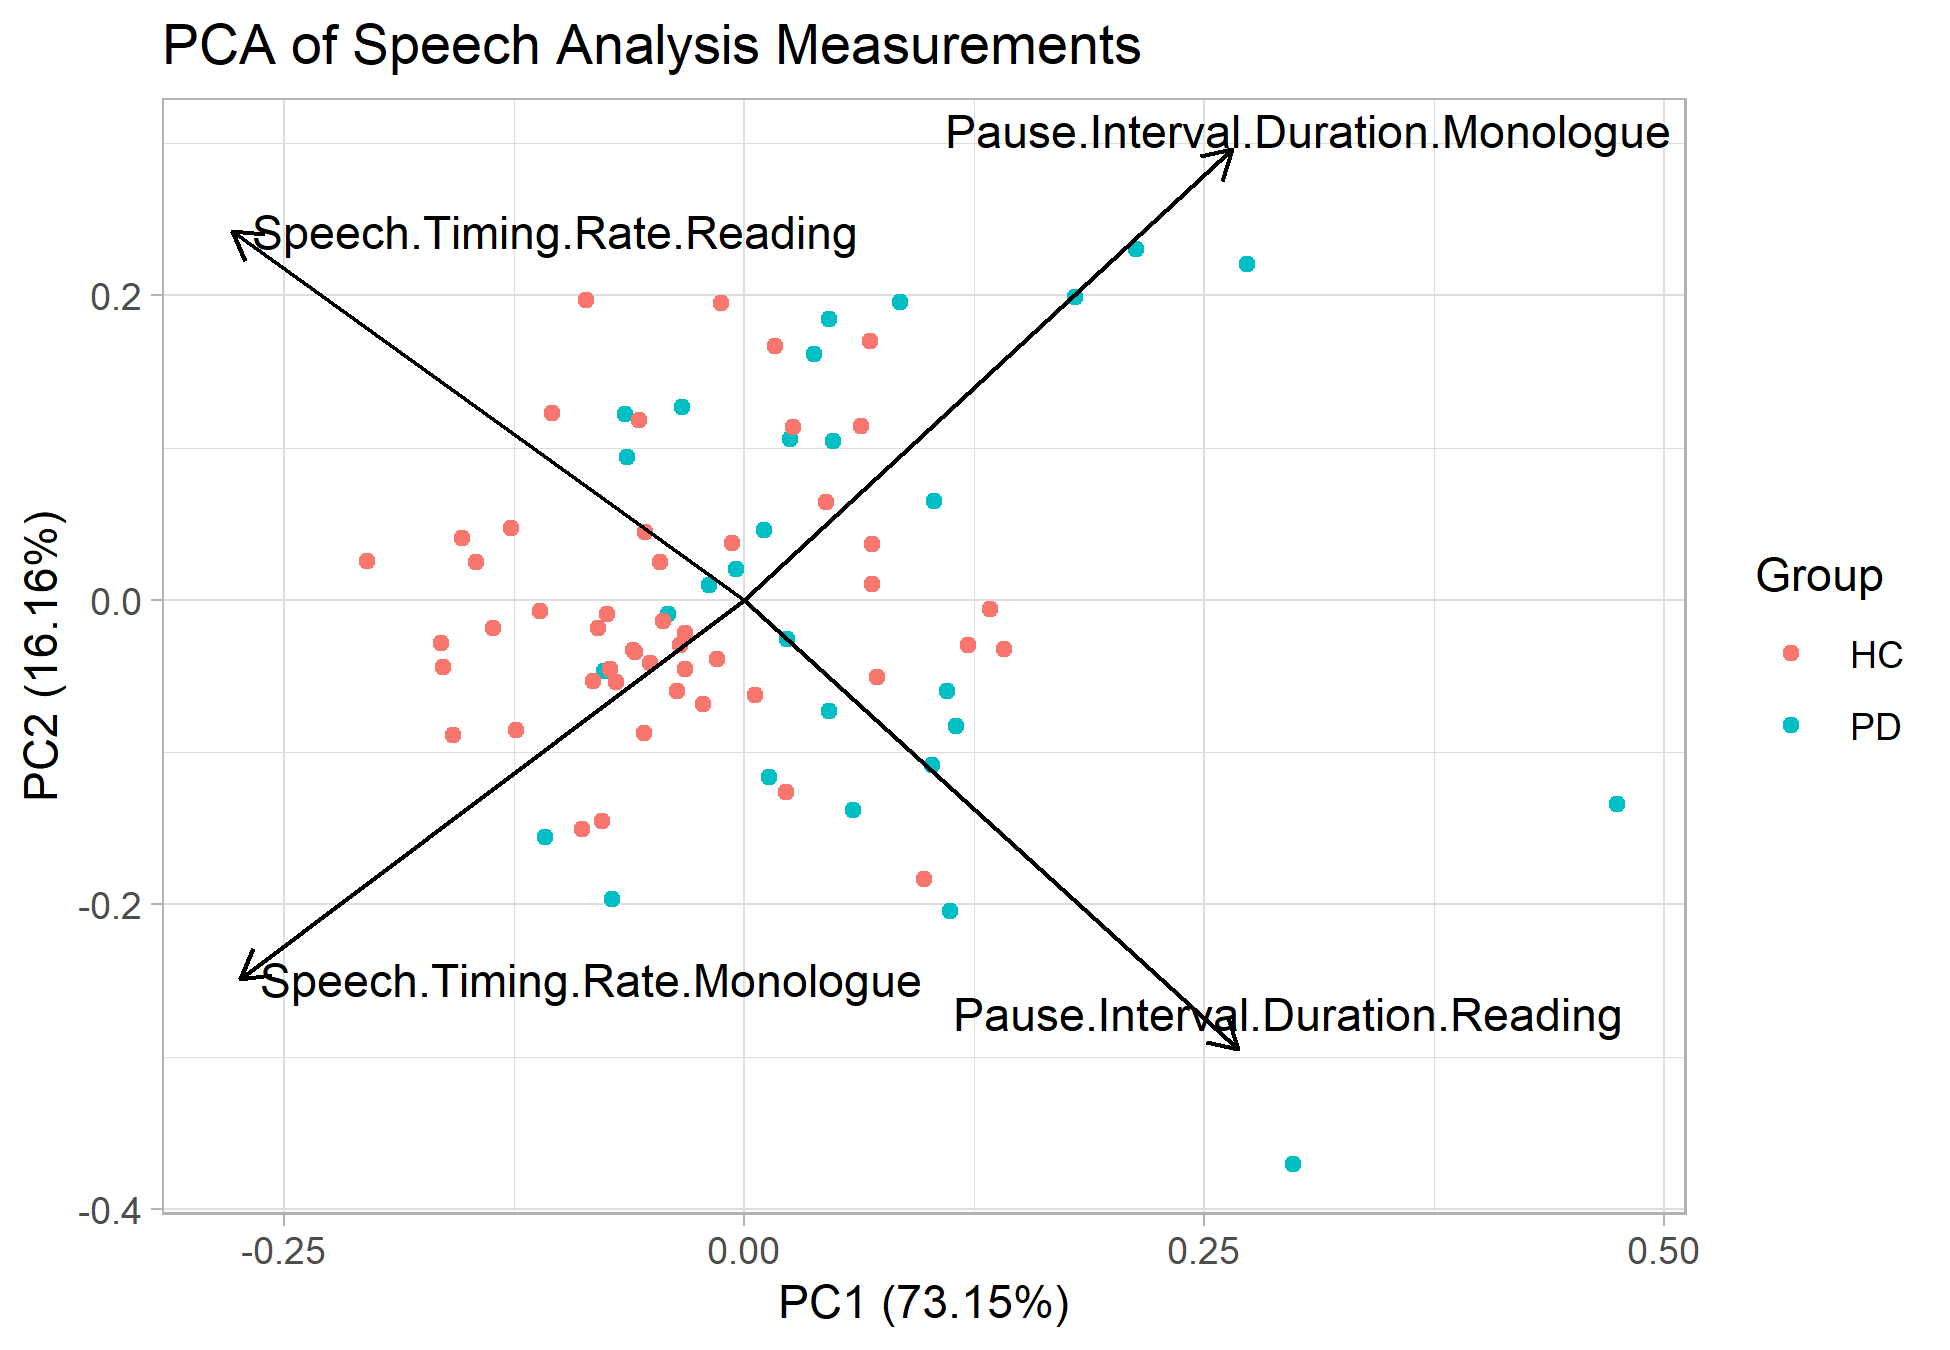
\includegraphics{dap_report_anja_probst_files/figure-latex/pca-loadings-1} 

}

\caption{PCA autoplot of PCs 1 and 2. It once again shows that there exists a strong correlation between the variables.}\label{fig:pca-loadings}
\end{figure}

Figure \ref{fig:pca-ggpairs} shows, that the PCA has resolved the correlations between the variables.

\begin{figure}
\centering
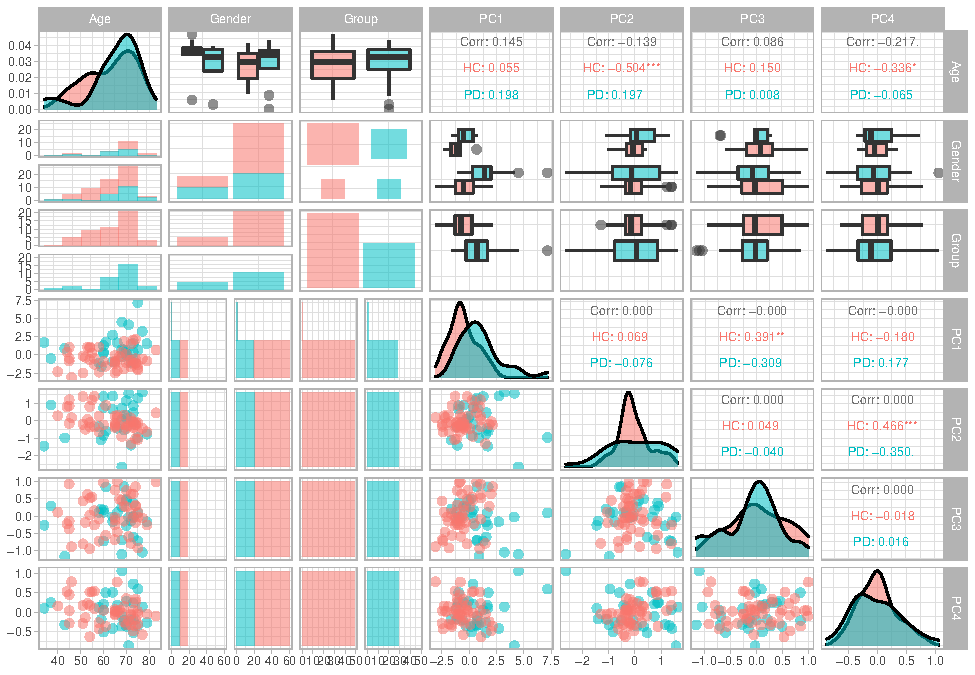
\includegraphics{dap_report_anja_probst_files/figure-latex/pca-ggpairs-1.pdf}
\caption{\label{fig:pca-ggpairs}ggpairs plot where the speech-related variables have been replaced by the principal components of a PCA.}
\end{figure}

A comparison between the interaction model with a model based on PC1 and the variable gender,
does not show a significant difference.

\begin{verbatim}
Analysis of Deviance Table

Model 1: Group ~ PC1 + Gender
Model 2: Group ~ Pause.Interval.Duration.Reading:Pause.Interval.Duration.Monologue + 
    Gender
  Resid. Df Resid. Dev Df Deviance Pr(>Chi)
1        75     77.765                     
2        75     77.694  0    0.071         
\end{verbatim}

\hypertarget{multinomial-regression}{%
\subsection{Multinomial Regression}\label{multinomial-regression}}

To predict over all three groups (HC, PD, RBD), we have to use a more complex
multinomial model. In order to evaluate the multinomial model, I created a train and test set. The training set contains 70\% of the observations, while the test set contains the
remaining 30\%.
Using the formula \texttt{Group\ \textasciitilde{}\ .\ -\ Age\ -\ Gender} results in the best performance.

\begin{Shaded}
\begin{Highlighting}[]
\CommentTok{\# Set reference level explicitly}
\NormalTok{df}\SpecialCharTok{$}\NormalTok{Group }\OtherTok{\textless{}{-}} \FunctionTok{relevel}\NormalTok{(df}\SpecialCharTok{$}\NormalTok{Group, }\AttributeTok{ref =} \StringTok{"HC"}\NormalTok{)}

\CommentTok{\# Train / test split}
\FunctionTok{set.seed}\NormalTok{(}\DecValTok{123}\NormalTok{)}
\NormalTok{sample }\OtherTok{\textless{}{-}} \FunctionTok{sample.int}\NormalTok{(}
    \AttributeTok{n =} \FunctionTok{nrow}\NormalTok{(df), }\AttributeTok{size =} \FunctionTok{floor}\NormalTok{(}\FloatTok{0.7} \SpecialCharTok{*} \FunctionTok{nrow}\NormalTok{(df)),}
    \AttributeTok{replace =} \ConstantTok{FALSE}
\NormalTok{)}

\NormalTok{df.train }\OtherTok{\textless{}{-}}\NormalTok{ df[sample, ]}
\NormalTok{df.test }\OtherTok{\textless{}{-}}\NormalTok{ df[}\SpecialCharTok{{-}}\NormalTok{sample, ]}

\NormalTok{model.all }\OtherTok{\textless{}{-}} \FunctionTok{multinom}\NormalTok{(}
\NormalTok{    Group }\SpecialCharTok{\textasciitilde{}}\NormalTok{ . }\SpecialCharTok{{-}}\NormalTok{ Age }\SpecialCharTok{{-}}\NormalTok{ Gender,}
    \AttributeTok{data =}\NormalTok{ df.train}
\NormalTok{)}
\end{Highlighting}
\end{Shaded}

\begin{verbatim}
# weights:  18 (10 variable)
initial  value 97.776494 
iter  10 value 78.995920
iter  20 value 77.591907
final  value 77.591844 
converged
\end{verbatim}

\begin{Shaded}
\begin{Highlighting}[]
\NormalTok{df.train}\SpecialCharTok{$}\NormalTok{Group.Predicted }\OtherTok{\textless{}{-}} \FunctionTok{predict}\NormalTok{(}
\NormalTok{    model.all,}
    \AttributeTok{newdata =}\NormalTok{ df.train, }\StringTok{"class"}
\NormalTok{)}

\NormalTok{tab }\OtherTok{\textless{}{-}} \FunctionTok{table}\NormalTok{(df.train}\SpecialCharTok{$}\NormalTok{Group, df.train}\SpecialCharTok{$}\NormalTok{Group.Predicted)}
\NormalTok{tab}
\end{Highlighting}
\end{Shaded}

\begin{verbatim}
     
      HC PD RBD
  HC  30  0   7
  PD   5  2  10
  RBD 11  1  23
\end{verbatim}

\begin{Shaded}
\begin{Highlighting}[]
\CommentTok{\# nicer way ot output a confusion matrix}
\CommentTok{\# calculate ratios instead of raw number to asses if True positive and false negative are high/low ? \# check Lucile\textquotesingle{}s DAP}
\NormalTok{accuracy }\OtherTok{\textless{}{-}} \FunctionTok{round}\NormalTok{((}\FunctionTok{sum}\NormalTok{(}\FunctionTok{diag}\NormalTok{(tab)) }\SpecialCharTok{/} \FunctionTok{sum}\NormalTok{(tab)) }\SpecialCharTok{*} \DecValTok{100}\NormalTok{, }\DecValTok{2}\NormalTok{)}
\end{Highlighting}
\end{Shaded}

The performance of this simple model is 61.80\%, this is especially interesting when inspecting the
confusion matrix above. None of the healthy subjects were diagnosed with Parkinson's disease, which is discrimination
important in a clinical setting. However, only 2 out of 17
subjects with PD were diagnosed correctly. In
addition, only 1 out of 35 subjects with RBD was misdiagnosed with PD.

\hypertarget{conclusion}{%
\section{Conclusion}\label{conclusion}}

Given the challenging nature of the data set, as well as the collinearity within it, the multinomial model
yielded surprisingly good performance by showing high specifity when diagnosing REM sleep behavior disorder
subjects and healthy controls. However, the logistic model, tasked with discriminating between
healthy controls and subjects suffering from Parkinson's Disease, did not express satisfactory performance. Chosing
difference combinations of predictors only had a small influence on the outcome. While I attribute this to
the highly correlated predictors, a PCA-based model could not improve the situation and did not result in
significantly better performance.

\clearpage

\hypertarget{manual-model-plot}{%
\subsection{Manual Model Plot}\label{manual-model-plot}}

\clearpage

\hypertarget{references}{%
\section{References}\label{references}}

\begingroup
\setlength{\parindent}{-0.5in}
\setlength{\leftskip}{0.5in}

\hypertarget{refs}{}
\begin{CSLReferences}{0}{0}
\end{CSLReferences}

\endgroup


\end{document}
